%!TEX root = CS818_assessment.tex
Supervised learning is a machine learning technique that uses labelled data to build predictive models. Decision tree analysis is one such supervised method, whereby an algorithm learns a sequence of decision rules to classify or predict outcomes based on input features. Decision trees work by iteratively partitioning a dataset, using a predictor variable and a criterion such as variance reduction as the basis for determining where to split the data. This process continues until a stopping criterion such as a maximum number of splits is reached \cite{Geron2022}. 

Similar to cluster analysis, decision tree analysis can simultaneously evaluate multiple variables. However, whilst K-Means analysis has been used to uncover latent groupings in the data, a decision tree will instead permit identification of key predictors. This can further refine our understanding of obesity risk's key drivers and their interactions.

\section{Decision Tree Analysis: results}

The analysis was run three times. First, it was completed for the full dataset. As can be seen in \ref{tab:decision_tree}, this achieved a strong accuracy score of 0.93, however the most important feature by a significant margin was 'Weight', followed by 'Height'. Given that weight is the primary determinant of BMI, it is dominating the model and overshadowing the potential predictive power of other factors. For the second run, 'Height' and 'Weight' were excluded to reduce the impact of body-measurement data on the results. Similarly, 'Age' and 'Gender' were excluded to focus specifically on lifestyle factors. The interplay between demographic features and obesity can be instructive for identifying high-risk groups. However, in focusing in on lifestyle factors, the analysis may identify behaviours that are within individuals' power to change. This model achieved an accuracy of 0.75, and the clusters were identified as the most important feature. The third and final run removed clusters to focus solely on lifestyle factors, and achieved an accuracy of 0.71. Such a small decline in accuracy indicates that whilst the clusters have helped identify groupings in the data, they do not have significant predictive power.

\begin{table}[htbp]
    \centering
    \caption{Comparison of Decision Tree Runs: Accuracy and Top 5 Features}
    \label{tab:decision_tree}
    
    % Run 1
    \begin{subtable}[t]{0.25\textwidth}
        \centering
        \caption{Run 1: 0.93}
        \begin{tabular}{ll}
            \toprule
            Feature & Imp \\
            \midrule
            Weight & 0.555 \\
            Height & 0.169 \\
            FCVC & 0.146 \\
            Age & 0.030 \\
            FAVC & 0.024 \\
            \bottomrule
        \end{tabular}
    \end{subtable}
    \hfill
    % Run 2
    \begin{subtable}[t]{0.25\textwidth}
        \centering
        \caption{Run 2: 0.75}
        \begin{tabular}{ll}
            \toprule
            Feature & Imp \\
            \midrule
            Cluster & 0.196 \\
            FCVC & 0.149 \\
            TUE & 0.097 \\
            FAF & 0.097 \\
            NCP & 0.096 \\
            \bottomrule
        \end{tabular}
    \end{subtable}
    \hfill
    % Run 3
    \begin{subtable}[t]{0.25\textwidth}
        \centering
        \caption{Run 3: 0.71}
        \begin{tabular}{ll}
            \toprule
            Feature & Imp \\
            \midrule
            TUE & 0.158 \\
            FCVC & 0.154 \\
            CH20 & 0.128 \\
            NCP & 0.111 \\
            FAF & 0.100 \\
            \bottomrule
        \end{tabular}
    \end{subtable}

\end{table}

The full list of variables and their importance in this final run is captured in \ref{fig:feature_importance}, and shows the most significant features were TUE (time on devices) and FCVC (vegetable consumption). The effectiveness of the model itself is captured in the classification report in table \ref{tab:classification_report}. A decision was made not to set a max depth for the decision tree to allow the model to capture more complex patterns. However, this can also increase the risk of overfitting. Looking at the classification report, while some classes, notably Obesity Type I, show lower recall and F1-scores, the overall balanced performance - with an accuracy of 0.71 and similar macro and weighted averages — suggests the model is not severely overfitting. This gives confidence that the model is capturing meaningful patterns across most classes rather than just memorizing the training data. 

\begin{table}[h]
\centering
\begin{tabular}{lcccc}
\toprule
\textbf{Class} & \textbf{Precision} & \textbf{Recall} & \textbf{F1-score} & \textbf{Support} \\
\midrule
Normal\_Weight      & 0.75 & 0.77 & 0.76 & 179 \\
Obesity\_Type\_I     & 0.64 & 0.58 & 0.61 & 102 \\
Obesity\_Type\_II    & 0.77 & 0.83 & 0.80 & 88  \\
Obesity\_Type\_III   & 0.94 & 0.98 & 0.96 & 98  \\
Overweight\_Level\_I & 0.52 & 0.48 & 0.50 & 88  \\
Overweight\_Level\_II& 0.53 & 0.54 & 0.54 & 79  \\
\midrule
Accuracy            &      &      & 0.71 & 634 \\
Macro Avg           & 0.69 & 0.70 & 0.69 & 634 \\
Weighted Avg        & 0.71 & 0.71 & 0.71 & 634 \\
\bottomrule
\end{tabular}
\caption{Classification Report}
\label{tab:classification_report}
\end{table}

\begin{figure}[h]
    \centering
    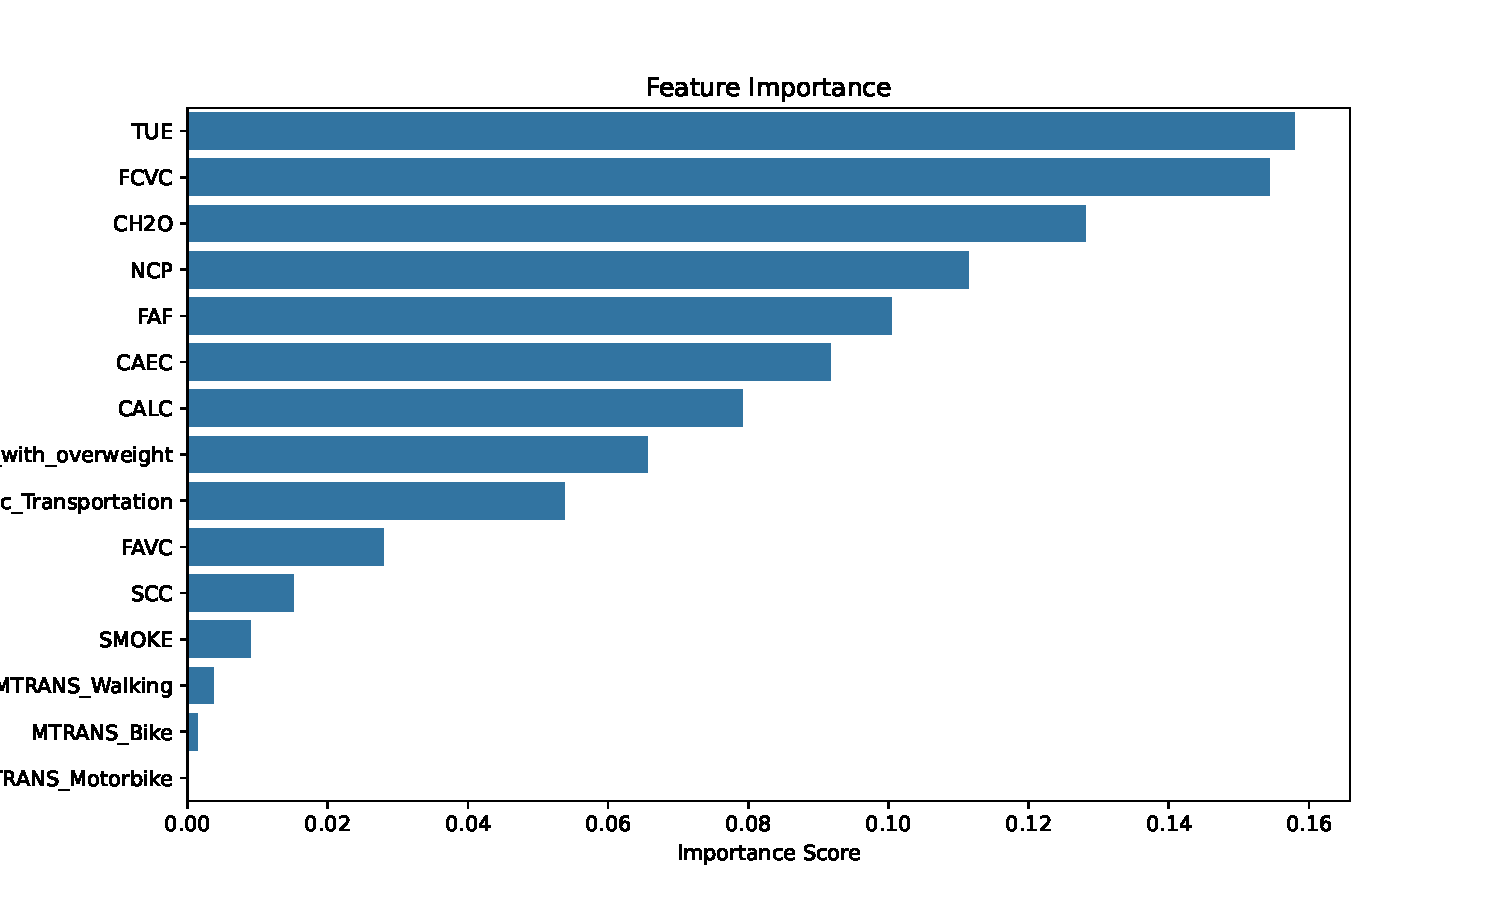
\includegraphics[width=1\textwidth]{feature_importance.pdf}
    \caption{Feature Importance Plot for Final Decision Tree}
    \label{fig:feature_importance}
\end{figure}


